\chapter{Implementation}
The implementation of the discussed methods for solving the heat equation and for model order reduction was done in Matlab.
Matlab was chosen as the programming language because it natively features matrix multiplication which finds heavy use in the previously mentioned methods.
The second reason for this selection is that there exist ToolBoxes that already implement certain model order reduction methods such as MORLAB \cite{benner_werner} or MOR toolbox \cite{MORT}.
The following figure shows the class diagram of the implementation:
\newline

\begin{figure}[H]
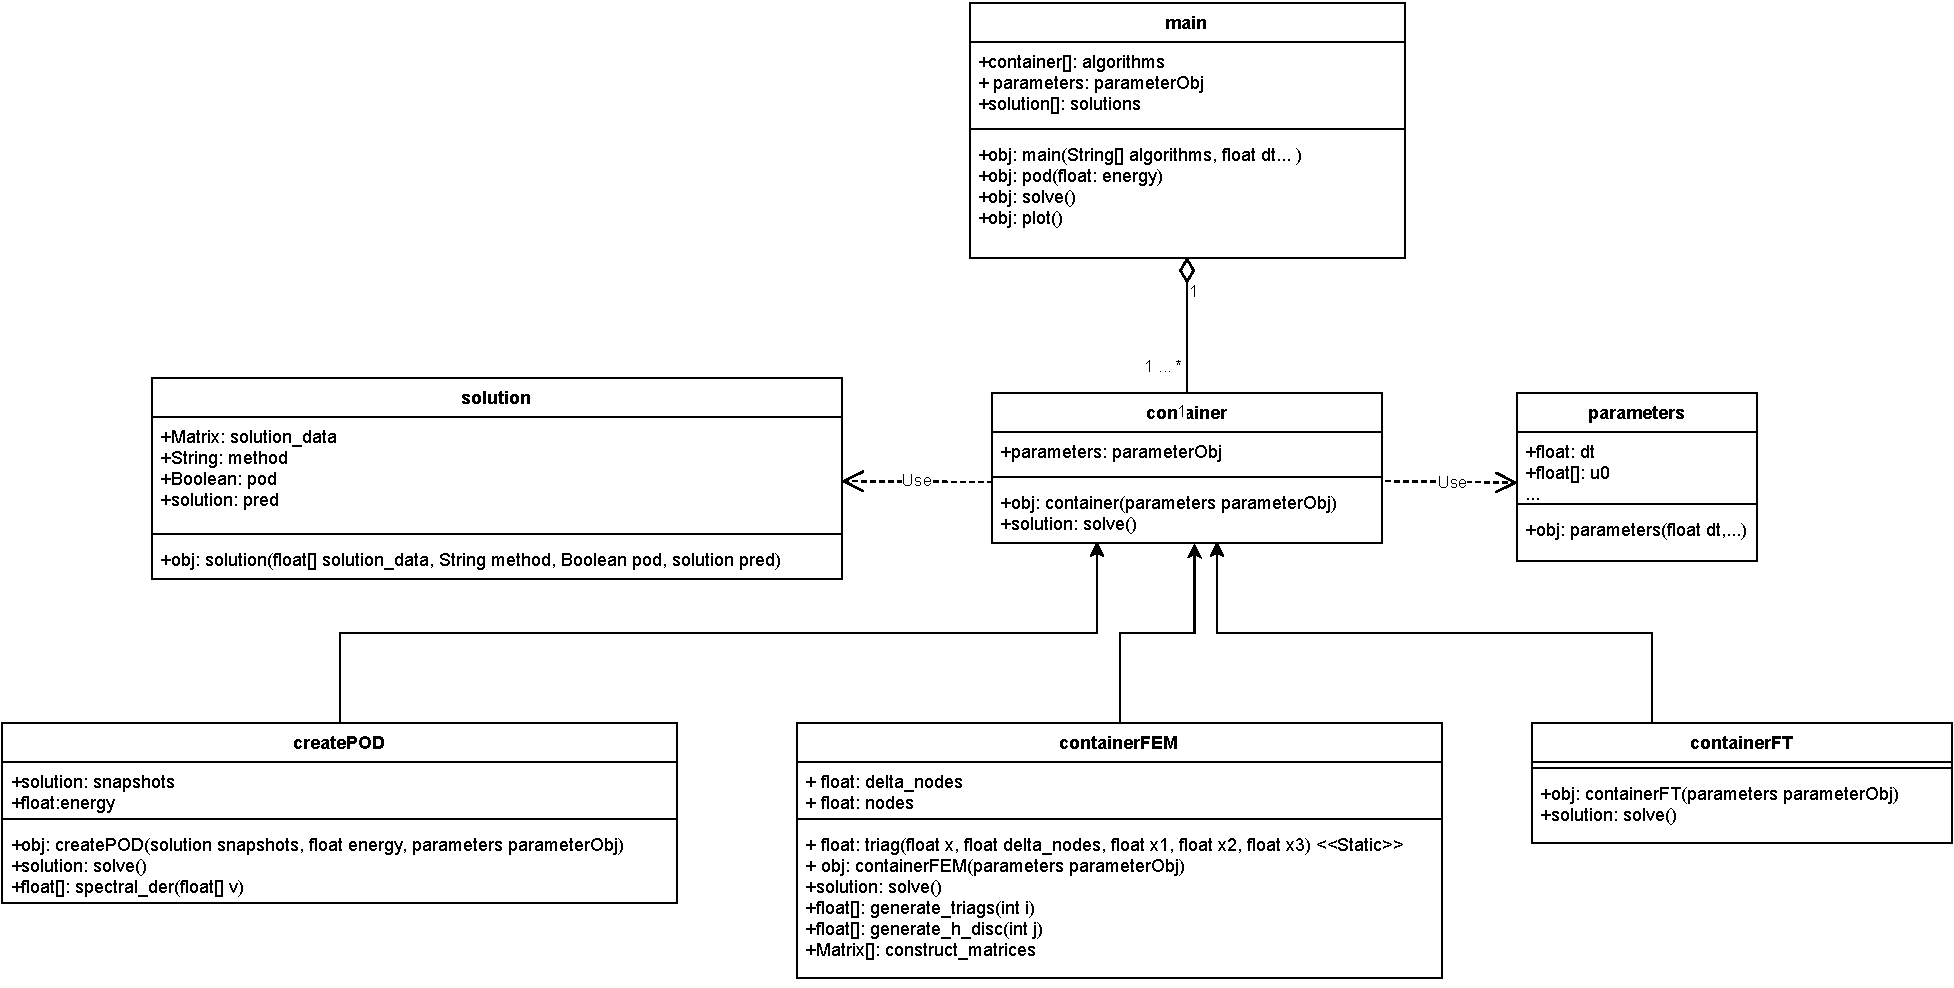
\includegraphics[ width=\textwidth]{images/class}
\caption{Class diagramm of MOR and FEM implementation}
\end{figure}
\section{Class main}
The class main is responsible for generating the finite element solution, model order reduction steps and plotting the results. The process can be seen in the following flow chart:
\begin{figure}[H]
\centering
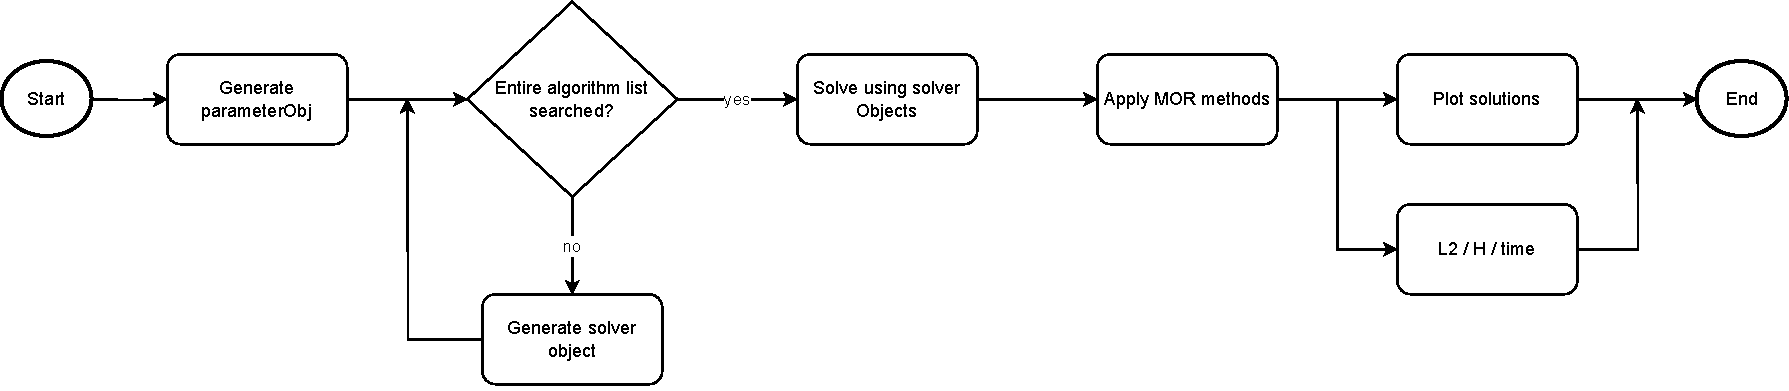
\includegraphics[ width=\textwidth]{images/main-seq}
\caption{Flow chart of main class}
\end{figure}
The first step is to generate a parameter object.
The parameter object stores all parameters in order to increase the transparency and robustness of the program.
The second step is to iterate the array of stated algorithms to solve the heat equation.
The options are to solve the heat equation using finite element method \ref{FEM} or using Fourier transform \ref{HE}.
After all solver objects have been generated, the according solutions are being computed.
After that, the MOR methods are displayed.
The final step is to display the solutions.
\section{Class containerFEM}
The class containerFEM is responsible for generating a solution using finite element method.
FEM is implemented in the following way:

\begin{figure}[H]
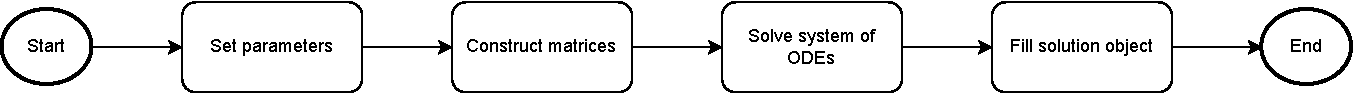
\includegraphics[ width=\textwidth]{images/seq-fem}
\caption{Flow chart for FEM class}
\end{figure}

The first step is to set the parameters.
After that the matrices discussed in \ref{FEM} are being constructed.
The next step is to solve the resulting system of ODEs and pass the solution to a solution object.
\subsection{Construct Matrices}
As defined in \ref{def-mat-a}  the matrices \(K\) and \(M\) have to be constructed.
Also to compute the initial condition given by \(u_0\) \(F\) has to be known \ref{F}.
This is done by the following method:
\begin{algorithm}[H]
\caption{Construct matrices \(K\), \(M\) and \(F\)}
\begin{algorithmic}[1]
\State $ii \gets \frac{2}{3} \Delta nodes$
\State $ij \gets \frac{1}{6} \Delta nodes$
\State $F \gets zeros(nodes, 1)$
\State $K \gets zeros(nodes)$
\State $M \gets zeros(nodes)$
\For{$i=1  \; \textbf{to} \; nodes$}
\State $F(i) \gets trapz(\phi_i \cdot u_0)$
\EndFor 
\For{$i=1  \; \textbf{to} \; nodes$}
\State $ K(i, i) \gets \frac{-2}{\Delta nodes}$
\State $ M(i, i) \gets ii$
\If{$i-1 > 1$}
\State $ K(i, i-1) \gets \frac{1}{\Delta nodes}$
\State $ M(i, i-1) \gets ij$
\EndIf
\If{$i+1 < nodes + 1$}
\State $ K(i, i+1) \gets \frac{1}{\Delta nodes}$
\State $ M(i, i+1) \gets ij$
\EndIf
\EndFor 
\State $\textbf{return} [F, K, M]$
\end{algorithmic}
\end{algorithm}

\subsection{Compute Vector d(t)}
As discussed in \ref{FEM} vector \(d\) has to be computed for each time step:
\begin{algorithm}[H]
\caption{Construct vector d}
\begin{algorithmic}[1]
\State $d \gets zeros(nodes, 1)$
\For{$i=1  \; \textbf{to} \; nodes$}
\State $d(i) \gets trapz(\phi_i \cdot h(x, t_0))$
\EndFor 
\State $\textbf{return } d$
\end{algorithmic}
\end{algorithm}
The entries of vector \(d\) become the integral of the product  of a basis function and \(h\) evaluated at time step \(t_0\).
This time step is a argument of that method.

\subsection{Solve System of ODEs}
The most important step in the process of generating a solution is to solve the system of ordinary differential equations that FEM yields:
\begin{algorithm}[H]
\caption{Solve system of ODEs using euler scheme}
\begin{algorithmic}[1]
\State $[F, K, M] \gets \textit{construct\_matrices()}$
\State $C \gets zeros(nodes, n\_time\_steps)$
\State $c_{0} \gets M^{-1}F$
\State $C(:, 1) \gets c_{0}$
\State $M(1, :) \gets [0, \hdots, 0]$
\State $M(end, :) \gets [0, \hdots, 0]$
\State $N \gets M^{-1}K$
\For{$t=2  \; \textbf{to} \; n\_time\_steps$}
\State $d \gets \textit{generate\_h\_disc(t)}$
\State $c_{n} \gets \Delta t N c_{0} + M^{-1} h + c_{0} $
\State $c_{0} \gets c_{n}$
\State $C(:, t) \gets c_{n}$
\EndFor
\State $S \gets []$
\For{$t=1  \; \textbf{to} \; n\_time\_steps$}
\State $c \gets C(:, t)$
\State $\textit{interpol} \gets \textit{interp1(linspace(0, L, nodes),c, X)}$
\State $S(:, t) \gets \textit{interpol}$
\EndFor
\State $\textbf{return } \textit{solution(S, "FEM", 0, 0)}$
\end{algorithmic}
\end{algorithm}
In the first line the matrices \(F\), \(K\) and \(M\) are retrieved.
After that the initial vector of coefficients \(c_0\) is computed using LS \ref{c0} in line three.
The next two following lines force the boundary conditions as stated in \ref{force-bound}.
In the lines 8 to 13 \ref{fem-euler} is implemented.
In the last step the coefficients are interpolated in spatial direction to fit the given domain \(X\) and stored in a solution object.


	



